\chapter{Implementacija i korisničko sučelje}


\section{Korištene tehnologije i alati}

Komunikacija u timu realizirana je korištenjem aplikacije \underline{Discord}\footnote{https://discord.com/}. Za izradu UML dijagrama korišten je alat \underline{Astah Professional}\footnote{https://astah.net/products/astah-professional/}, a kao sustav za upravljanje izvornim kodom \underline{Git}\footnote{https://git-scm.com/}. Udaljeni repozitorij projekta je dostupan na web platformi \underline{GitHub}\footnote{https://github.com/}.

Kao razvojno okruženje korišten je \underline{IntelliJ IDEA}\footnote{https://www.jetbrains.com/idea/} - integrirano je razvojno \newline okruženje (IDE) tvrtke JetBrains. Prvenstveno se koristi za razvoj računalnih programa za operacijski sustav Windows, kao i za web-stranice, web-aplikacije, web-usluge i mobilne aplikacije. IntelliJ IDEA za razvoj softvera koristi JetBrains platforme i tehnologije za olakšavanje procesa razvoja. To uključuje podršku za razvoj u raznim programskim jezicima(poput Java, Kotlin, Groovy i mnogih drugih), za Android razvoj, Spring Framework, Web development(\textit{frontend} i \textit{backend}) itd. Uz IntelliJ IDEA ponešto je korišten i \underline{Visual Studio Code}\footnote{https://code.visualstudio.com/}, ali uglavnom kao text editor te za pisanje \underline{docker}\footnote{https://www.docker.com/} deploy skripte. Docker predstavlja platformu kao uslugu(Paas) koja koristi virtualizaciju na razini OS-a za isporuku programa u spremnicima. Spremnici osiguravaju izolaciju procesa, mreže i datotečnog sustava.

Aplikacija je napisana koristeći radni okvir \underline{Spring Framework}\footnote{https://spring.io/} i jezik \underline{Java}\footnote{https://www.java.com/en/} za izradu \textit{backenda} te \underline{React}\footnote{https://react.dev/} i jezik \underline{TypeScript}\footnote{https://www.typescriptlang.org/} za izradu \textit{frontenda}. React, također poznat kao React.js ili ReactJS, je biblioteka u JavaScriptu za izgradnju korisničkih sučelja. Održavana je od strane Facebooka. React se najčešće koristi kao osnova u razvoju web ili mobilnih aplikacija. Složene aplikacije u Reactu obično zahtijevaju korištenje dodatnih biblioteka za interakciju s API-jem. Programski jezik TypeScript je nadogradnja na JavaScript, a napravio ga je Microsoft. Radni okvir Spring Framework nadograđuje mogućnosti samog operativnog sustava. Radi se o posebnoj infrastrukturi koja programerima nudi gotova rješenja i funkcionalnosti da bi ubrzala i pojednostavila razvoj aplikacija svih vrsta i oblika.

Baza podataka se nalazi na poslužitelju u oblaku \underline{Render}\footnote{https://render.com/}.

\eject


\section{Ispitivanje programskog rješenja}

\textbf{\textit{dio 2. revizije}}\\

\textit{U ovom poglavlju je potrebno opisati provedbu ispitivanja implementiranih funkcionalnosti na razini komponenti i na razini cijelog sustava s prikazom odabranih ispitnih slučajeva. Studenti trebaju ispitati temeljnu funkcionalnost i rubne uvjete.}

\subsection{Ispitivanje komponenti}
Ispitivanje komponenti sustava smo proveli uz pomoć alata \underline{JUnit} \footnote{https://junit.org/junit5/}, okvira za jedinično testiranje za programski jezik Java koji je iznimno važan u razvoju vođenom testiranjem. Pri razvoju aplikacije korištena je inačica 5.

\text{Izvorni kôd svih ispitnih slučajeva i rezultati izvođenja ispita prikazani su u nastavku}
\renewcommand{\lstlistingname}{Kod}
\begin{lstlisting}[
	language=Java,
	frame=single,
	label={lst:testGetAllRequestedAdvertisements},
	basicstyle = \small,
	tabsize=2,
	showspaces=false,
	showstringspaces=false,
	commentstyle = \color{red}, %% set comment color
	keywordstyle = \color{blue}, %% set keyword color
	stringstyle = \color{applegreen}, %% set string color
	rulecolor = \color{black},
	caption={Test testGetAllRequestedAdvertisements},
	breaklines=true]
	@Test
	@DisplayName("All requested advertisements are fetched")
	public void testGetAllRequestedAdvertisements() {
		
		Advertisement advertisement1 = mock(Advertisement.class);
		when(advertisement1.getAdState()).thenReturn(AdStateEnum.ACTIVE);
		when(advertisement1.getCategory()).thenReturn(CategoryEnum.LJUBIMAC_JE_SRETNO_PRONADEN);
		
		Advertisement advertisement2 = mock(Advertisement.class);
		when(advertisement2.getAdState()).thenReturn(AdStateEnum.ACTIVE);
		when(advertisement2.getCategory()).thenReturn(CategoryEnum.LJUBIMAC_JE_NESTAO_I_ZA_NJIM_SE_TRAGA);
		when(advertisement2.getPet()).thenReturn(mock(Pet.class));
		when(advertisement2.getUser()).thenReturn(mock(Registered.class));
		when(imageRepository.findAllByPetPetId(anyLong())).thenReturn(Arrays.asList(mock(Image.class)));
		
		when(advertisementRepository.findAll()).thenReturn(Arrays.asList(
		advertisement1, advertisement2)
		);
		
		List<AdvertisementSummaryDTO> result = advertisementService.getAllAdvertisements(
		CategoryEnum.LJUBIMAC_JE_NESTAO_I_ZA_NJIM_SE_TRAGA
		);
		
		assertEquals(1, result.size());
	}
\end{lstlisting}

U Kodu \ref{lst:testGetAllRequestedAdvertisements} prikazuje se ispitni slučaj koji osigurava da metoda AdvertisementService.getAllAdvertisements(CategoryEnum category) ispravno dohvaća i vraća oglase koji odgovaraju zadanom kriteriju kategorije. Kreiraju se dva mock (simulirana) oglasa (advertisement1 i advertisement2) koristeći Mockito okvir za testiranje. Oba oglasa su postavljena na aktivno stanje (AdStateEnum.ACTIVE), ali pripadaju različitim kategorijama. S obzirom da samo 1 objekt pripada traženoj kategoriji (advertisement2), sa assertEquals(1, result.size()) provjeravamo jesmo li dobili samo 1 oglas.

\pagebreak

\begin{lstlisting}[
	language=Java,
	frame=single,
	label={lst:testNoneAdsOfRequestedCategoryFound},
	basicstyle = \small,
	tabsize=2,
	showspaces=false,
	showstringspaces=false,
	commentstyle = \color{red}, %% set comment color
	keywordstyle = \color{blue}, %% set keyword color
	stringstyle = \color{applegreen}, %% set string color
	rulecolor = \color{black},
	caption={Test testNoneAdsOfRequestedCategoryFound},
	breaklines=true]
	@Test
	@DisplayName("Having zero advertisements of requested category is handled correctly")
	public void testNoneAdsOfRequestedCategoryFound() {
		
		Advertisement advertisement1 = mock(Advertisement.class);
		when(advertisement1.getAdState()).thenReturn(AdStateEnum.DELETED);
		
		Advertisement advertisement2 = mock(Advertisement.class);
		when(advertisement2.getAdState()).thenReturn(AdStateEnum.ACTIVE);
		when(advertisement2.getCategory()).thenReturn(CategoryEnum.LJUBIMAC_JE_SRETNO_PRONADEN);
		
		when(advertisementRepository.findAll()).thenReturn(Arrays.asList(
		advertisement1, advertisement2)
		);
		
		List<AdvertisementSummaryDTO> result = advertisementService.getAllAdvertisements(
		CategoryEnum.LJUBIMAC_JE_PRONADEN_U_NESRETNIM_OKOLNOSTIMA
		);
		
		assertEquals(0, result.size());
	}
\end{lstlisting}

U Kodu \ref{lst:testNoneAdsOfRequestedCategoryFound} prikazuje se ispitni slučaj koji, kao i u prethodnom ispitnom slučaju, ispituje funkcionalnost metode  AdvertisementService.getAllAdvertisements(CategoryEnum category), ali ovaj put ispitujemo rubni slučaj: u bazi ne postoji oglas koji ispunjava korisnički zadane kriterije (ili ne pripada traženoj kategoriji ili je "obrisan"). Sa assertEquals(0, result.size()) provjeravamo je li povratna vrijednost metode ispitivane metode prazna lista. 

\pagebreak

\begin{lstlisting}[
	language=Java,
	frame=single,
	label={lst:testRegisteredUserCannotSetInShelterCategory},
	basicstyle = \small,
	tabsize=2,
	showspaces=false,
	showstringspaces=false,
	commentstyle = \color{red}, %% set comment color
	keywordstyle = \color{blue}, %% set keyword color
	stringstyle = \color{applegreen}, %% set string color
	rulecolor = \color{black},
	caption={Test testRegisteredUserCannotSetInShelterCategory},
	breaklines=true]
	@Test
	@DisplayName("Non-shelter user cannot set U_SKLONISTU category")
	public void testRegisteredUserCannotSetInShelterCategory() {
		
		assertThrows(SecurityException.class, () -> {
			
			Long adId = 1L;
			AddAdvertisementDTO dto = mock(AddAdvertisementDTO.class);
			when(dto.getCategory()).thenReturn(CategoryEnum.U_SKLONISTU);
			when(dto.getDisappearanceLocationLat()).thenReturn(null);
			
			when(advertisementRepository.existsByAdvertisementId(anyLong())).thenReturn(true);
			
			Advertisement changedAdvertisement = mock(Advertisement.class);
			when(changedAdvertisement.getUser()).thenReturn(mock(Registered.class));
			
			when(advertisementRepository.findByAdvertisementId(anyLong())).thenReturn(Optional.of(changedAdvertisement));
			
			advertisementService.changeAdvertisement(adId, dto);
		});
	}
\end{lstlisting}

U Kodu \ref{lst:testRegisteredUserCannotSetInShelterCategory} nalazi se ispitni slučaj koji provjerava ispravnost rada metode AdvertisementService.changeAdvertisement(long adId, AddAdvertisementDTO dto). Testira se slučaj kada obični (registrirani) korisnik pokušava promijeniti svoj oglas tako da mu postavi kategoriju "U SKLONISTU". S obzirom da on nema dopuštenje za postavljanje te kategorije (nije sklonište), metoda changeAdvertisement() bi trebala baciti SecurityException iznimku, što i provjeravamo sa kodnim isječkom assertThrows(SecurityException.class, ...).

\pagebreak

\begin{figure}[!htb]
	\centering
	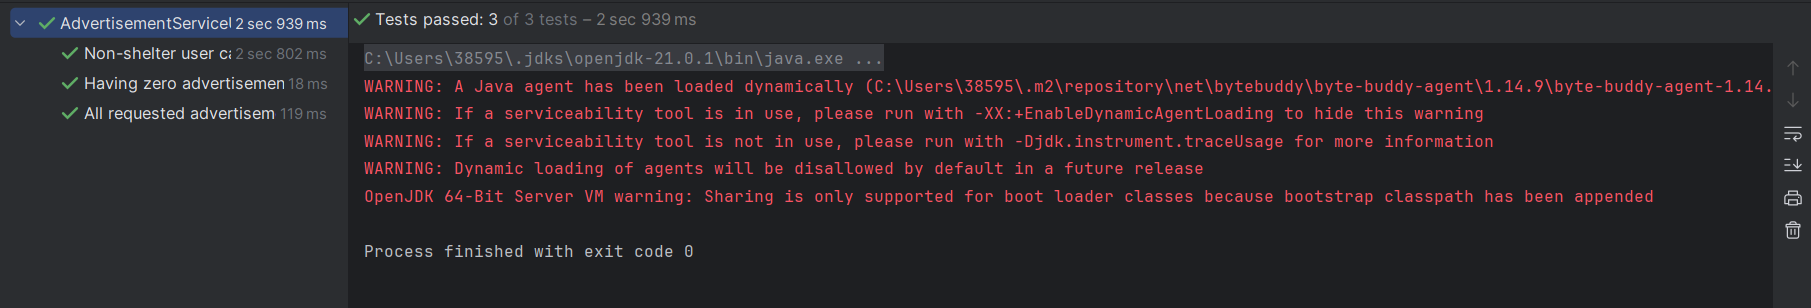
\includegraphics[width=\textwidth]{slike/test1.png}
	\caption{Testovi prolaze}
\end{figure}

\begin{lstlisting}[
	language=Java,
	frame=single,
	label={lst:testGetLocation},
	basicstyle = \small,
	tabsize=2,
	showspaces=false,
	showstringspaces=false,
	commentstyle = \color{red}, %% set comment color
	keywordstyle = \color{blue}, %% set keyword color
	stringstyle = \color{applegreen}, %% set string color
	rulecolor = \color{black},
	caption={Test testGetLocation},
	breaklines=true]
	@BeforeEach
	public void setup() {
		locationService = new LocationService(countyRepository, placeRepository, locationRepository) {
			@Override
			protected MapsSummaryDTO getLocInfoFromAPI(double latitude, double longitude) {
				MapsSummaryDTO dto = new MapsSummaryDTO();
				dto.setLocationName("Zagreb");
				dto.setPlace("Zagreb");
				dto.setCounty("Grad Zagreb");
				dto.setPostalCode("10000");
				return dto;
			}
		};
	}
	
	@Test
	@DisplayName("Location objects are retrieved successfully")
	public void testGetLocation() {
		when(countyRepository.existsByName(anyString())).thenReturn(true);
		when(countyRepository.findByName(anyString())).thenReturn(Optional.of(new County("Grad Zagreb")));
		when(placeRepository.existsByZipCode(anyLong())).thenReturn(true);
		when(placeRepository.findByZipCode(anyLong())).thenReturn(Optional.of(
		new Place(10000L, "Zagreb", new County("Grad Zagreb"))
		));
		
		locationService.getLocation(45.815399, 15.966568);
		
		Mockito.verify(locationRepository, times(1)).save(any(Location.class));
		
	}
\end{lstlisting}

U Kodu \ref{lst:testRegisteredUserCannotSetInShelterCategory} osigurava da metoda LocationService.getLocation(double latitude, double longitude) ispravno dohvaća informacije o lokaciji s API-ja, pravilno interagira s repozitorijima i sprema dobivene informacije o lokaciji. Test provjerava je li metoda save() pozvana nad objektom locationRepository točno jednom: ako je, to znači da je implementacija metode ispravna prema ovom scenariju, a ako nije, to ukazuje na potencijalni problem u implementaciji metode. NAPOMENA: s obzirom da povezivanje na API pri izvođenju unit testa nije preporučeno, metoda getLocInfoFromAPI(double latitude, double longitude) je konfigurirana da uvijek vraća informacije o lokaciji Zagreb, bez obzira na ulazne parametre. 

\begin{figure}[!htb]
	\centering
	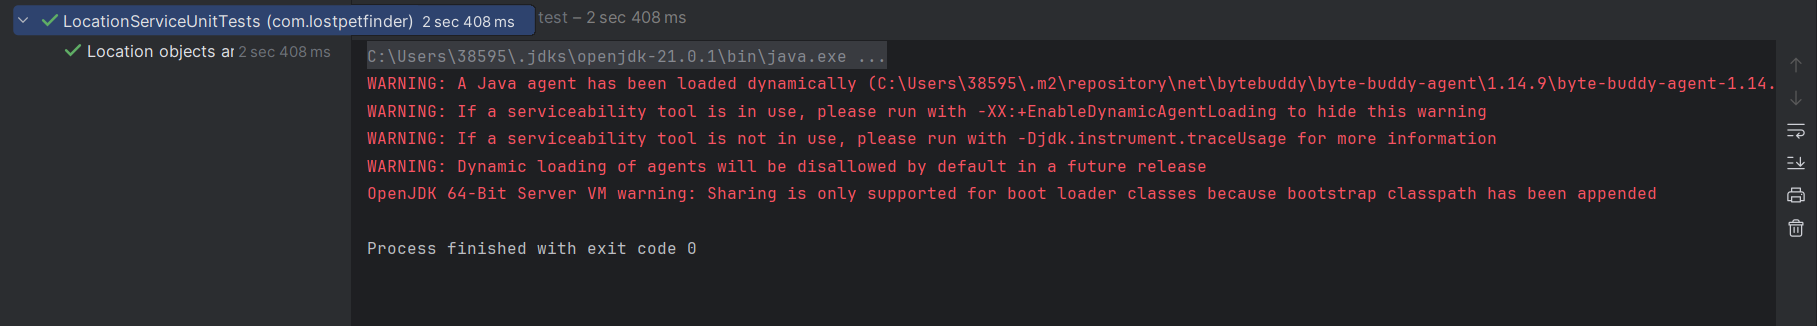
\includegraphics[width=\textwidth]{slike/test2.png}
	\caption{Test prolazi}
\end{figure}

\pagebreak

\begin{lstlisting}[
	language=Java,
	frame=single,
	label={lst:testSaveMessageWithTextOnly},
	basicstyle = \small,
	tabsize=2,
	showspaces=false,
	showstringspaces=false,
	commentstyle = \color{red}, %% set comment color
	keywordstyle = \color{blue}, %% set keyword color
	stringstyle = \color{applegreen}, %% set string color
	rulecolor = \color{black},
	caption={Test testSaveMessageWithTextOnly},
	breaklines=true]
	@Test
	@DisplayName("Messages with text only are successfully saved")
	public void testSaveMessageWithTextOnly() {
		
		MessageInputDTO dto = mock(MessageInputDTO.class);
		when(dto.getSenderUsername()).thenReturn("testUser");
		when(dto.getMessageText()).thenReturn("testMessageText");
		when(dto.getAdvertisementId()).thenReturn(1L);
		
		when(userRepository.findByUsername(anyString())).thenReturn(Optional.of(mock(User.class)));
		when(advertisementRepository.findByAdvertisementId(anyLong())).thenReturn(
		Optional.of(mock(Advertisement.class))
		);
		
		messageService.saveMessage(dto);
		
		Mockito.verify(messageRepository, times(1)).save(any(Message.class));
	}
\end{lstlisting}

U Kodu \ref{lst:testSaveMessageWithTextOnly} nalazi se ispitni slučaj koji  provjerava funkcionalnost metode MessageService.saveMessage(MessageInputDTO dto) kada je u sklopu poruke poslan tekst, ali ne i lokacija. Kreira se simulirani objekt MessageInputDTO pomoću metode mock() koji se zatim konfigurira da vrati “testUser” kao korisničko ime pošiljatelja, “testMessageText” kao tekst poruke i 1L kao ID oglasa. Metode findByUsername() u userRepository i findByAdvertisementId() u advertisementRepository su konfigurirane da uvijek vraćaju Optional objekt User i Advertisement, bez obzira na ulazne parametre. Metoda saveMessage se zatim poziva s prethodno kreiranim MessageInputDTO objektom. Na kraju, test provjerava je li metoda save() u messageRepository pozvana točno jednom.

\pagebreak

\begin{lstlisting}[
	language=Java,
	frame=single,
	label={lst:testSaveMessageWithLocationProvided},
	basicstyle = \small,
	tabsize=2,
	showspaces=false,
	showstringspaces=false,
	commentstyle = \color{red}, %% set comment color
	keywordstyle = \color{blue}, %% set keyword color
	stringstyle = \color{applegreen}, %% set string color
	rulecolor = \color{black},
	caption={Test testSaveMessageWithLocationProvided},
	breaklines=true]
	@Test
	@DisplayName("Messages with location included are successfully saved")
	public void testSaveMessageWithLocationProvided() {
		
		MessageInputDTO dto = mock(MessageInputDTO.class);
		when(dto.getSenderUsername()).thenReturn("testUser");
		when(dto.getMessageText()).thenReturn("testMessageText");
		when(dto.getAdvertisementId()).thenReturn(1L);
		when(dto.getDisappearanceLocationLat()).thenReturn(45.815399);
		when(dto.getDisappearanceLocationLng()).thenReturn(15.966568);
		
		when(userRepository.findByUsername(anyString())).thenReturn(Optional.of(mock(User.class)));
		when(advertisementRepository.findByAdvertisementId(anyLong())).thenReturn(
		Optional.of(mock(Advertisement.class))
		);
		when(locationRepository.existsByCoordinates(any(CoordinatesPK.class))).thenReturn(false);
		when(locationService.getLocation(anyDouble(), anyDouble())).thenReturn(mock(Location.class));
		
		messageService.saveMessage(dto);
		
		Mockito.verify(locationRepository, times(1)).save(any(Location.class));
		Mockito.verify(messageRepository, times(1)).save(any(Message.class));
	}
\end{lstlisting}

U Kodu \ref{lst:testSaveMessageWithLocationProvided} prikazuje se ispitni slučaj koji, kao i u prethodnom ispitnom slučaju, ispituje funkcionalnost metode MessageService.saveMessage(MessageInputDTO dto), ali u slučaju kada je lokacija zadana. Dio koda Mockito.verify(locationRepository, times(1)).save(any(Location.class)) provjerava je li pozvana metoda save() nad objektom locationRepository kako bi se utvrdilo da je zadana lokacija spremljena.

\pagebreak

\begin{lstlisting}[
	language=Java,
	frame=single,
	label={lst:testIfRetrievedChatMessagesAreOrdered},
	basicstyle = \small,
	tabsize=2,
	showspaces=false,
	showstringspaces=false,
	commentstyle = \color{red}, %% set comment color
	keywordstyle = \color{blue}, %% set keyword color
	stringstyle = \color{applegreen}, %% set string color
	rulecolor = \color{black},
	caption={Test testIfRetrievedChatMessagesAreOrdered},
	breaklines=true]
	@Test
	@DisplayName("Messages are retrieved in correct order")
	public void testIfRetrievedChatMessagesAreOrdered() {
		
		Message message1 = mock(Message.class);
		when(message1.getAltId()).thenReturn(new MessagePK(mock(User.class), LocalDateTime.now().minusDays(1)));
		when(message1.getAdvertisement()).thenReturn(mock(Advertisement.class));
		when(message1.getText()).thenReturn("Hello, World from testUser1!");
		
		Message message2 = mock(Message.class);
		when(message2.getAltId()).thenReturn(new MessagePK(mock(User.class), LocalDateTime.now()));
		when(message2.getAdvertisement()).thenReturn(mock(Advertisement.class));
		when(message2.getText()).thenReturn("Hello, World from testUser2!");
		
		when(messageRepository.findAllByAdvertisementAdvertisementId(anyLong())).thenReturn(
		Arrays.asList(message1, message2)
		);
		
		List<MessageDTO> result = messageService.getChatMessages(1L);
		
		assertEquals(2, result.size());
		assertEquals("Hello, World from testUser2!", result.get(0).getMessageText());
	}
\end{lstlisting}

U Kodu \ref{lst:testIfRetrievedChatMessagesAreOrdered} testira se vraća li metoda MessageService.getChatMessages(Long advertisementId) poruke za zahtijevani oglas u odgovarajućem poretku (prvo novije, zatim starije). Kreiraju se dva mock objekta: message1 (predstavlja stariju poruku) i message2 (predstavlja noviju poruku). Ako metoda getChatMessages() vrati 2 objekta tipa MessageDTO i ako je tekst prve poruke u vraćenoj listi "Hello, World from testUser2!", možemo zaključiti da metoda ispravno funkcionira.

\begin{figure}[!htb]
	\centering
	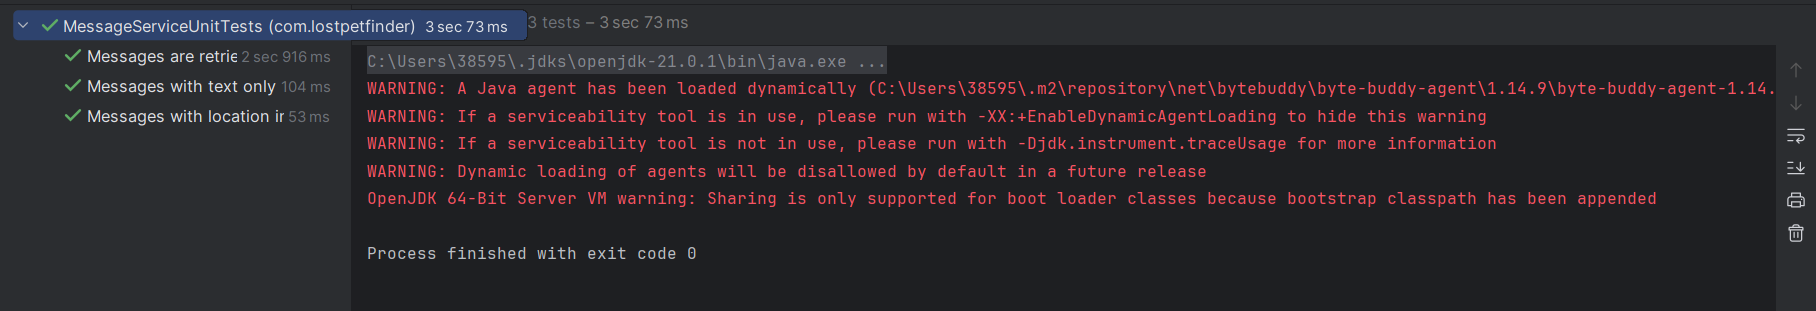
\includegraphics[width=\textwidth]{slike/test3.png}
	\caption{Testovi prolaze}
\end{figure}

\pagebreak

\subsection{Ispitivanje sustava}
\textit{Potrebno je provesti ispitivanje jedinica (engl. unit testing) nad razredima koji implementiraju temeljne funkcionalnosti. Razraditi \textbf{minimalno 6 ispitnih slučajeva} u kojima će se ispitati redovni slučajevi, rubni uvjeti te izazivanje pogreške (engl. exception throwing). Poželjno je stvoriti i ispitni slučaj koji koristi funkcionalnosti koje nisu implementirane. Potrebno je priložiti izvorni kôd svih ispitnih slučajeva te prikaz rezultata izvođenja ispita u razvojnom okruženju (prolaz/pad ispita). }

\subsection{Ispitivanje sustava}

Ispitivanje sustava proveli smo pomoću dodatka za preglednik
\underline{Selenium IDE} \footnote{https://www.selenium.dev/documentation/ide/}
te koristeći \underline{Selenium WebDriver}
\footnote{https://www.selenium.dev/documentation/webdriver/} unutar JUnit
testova.

\text{Ispitivanje pomoću Selenium WebDrivera prikazana su na slikama * i *}
\renewcommand{\lstlistingname}{Kod}
\begin{lstlisting}[
				language=Java,
				frame=single,
				label={lst:testLoginGoodCreds},
				basicstyle = \small,
				tabsize=2,
				showspaces=false,
				showstringspaces=false,
				commentstyle = \color{red}, %% set comment color
				keywordstyle = \color{blue}, %% set keyword color
				stringstyle = \color{applegreen}, %% set string color
				rulecolor = \color{black},
				caption={Test testLoginGoodCreds},
				breaklines=true]
@Test
public void testLoginGoodCreds() {
	WebDriver driver = new ChromeDriver();
	System.setProperty(
	"webdriver.chrome.driver", 
	"C:\\Users\\akrkl\\AppData\\Local\\Microsoft\\WindowsApps\\chromedriver.exe"
	);
	driver.manage().timeouts().implicitlyWait(10, TimeUnit.SECONDS);

	driver.get("http://localhost:5173/login");

	WebElement element = driver.findElement(By.id("email"));
	element.sendKeys("testadmin");

	element = driver.findElement(By.id("lozinka"));
	element.sendKeys("123");

	driver.findElement(By.cssSelector("button[type='submit']")).click();

	WebDriverWait wait = new WebDriverWait(driver, Duration.ofSeconds(2));
	try {
	wait.until(
		ExpectedConditions.presenceOfElementLocated(By.id("searchBarByCategories"))
	);

	String redirectUrl = driver.getCurrentUrl();

	Assertions.assertEquals(
		"http://localhost:5173/", redirectUrl
	);
	}
	finally {
	driver.quit();
	}
}	
			\end{lstlisting}

U Kodu \ref{lst:testLoginGoodCreds} testira se uspješan login korisnika. WebDriver otvara stranicu za login, pronalazi elemente za unos korisničkog imena i lozinke te unosi podatke. Nakon toga klikne na gumb za prijavu i čeka da se pojavi element za pretraživanje po kategorijama. Na kraju provjerava je li korisnik preusmjeren na početnu stranicu.

\pagebreak

\begin{lstlisting}[
				language=Java,
				frame=single,
				label={lst:testLoginBadCreds},
				basicstyle = \small,
				tabsize=2,
				showspaces=false,
				showstringspaces=false,
				commentstyle = \color{red}, %% set comment color
				keywordstyle = \color{blue}, %% set keyword color
				stringstyle = \color{applegreen}, %% set string color
				rulecolor = \color{black},
				caption={Test testLoginBadCreds},
				breaklines=true]
@Test
public void testLoginBadCreds() {
	WebDriver driver = new ChromeDriver();
	System.setProperty(
		"webdriver.chrome.driver",
		"C:\\Users\\akrkl\\AppData\\Local\\Microsoft\\WindowsApps\\chromedriver.exe"
	);
	driver.manage().timeouts().implicitlyWait(10, TimeUnit.SECONDS);
	driver.get("http://localhost:5173/login");

	WebElement element = driver.findElement(By.id("email"));
	element.sendKeys("testadmin");

	element = driver.findElement(By.id("lozinka"));
	element.sendKeys("wrongPassword");

	driver.findElement(By.cssSelector("button[type='submit']")).click();

	try {
		String redirectUrl = driver.getCurrentUrl();

		Assertions.assertNotEquals(
			"http://localhost:5173/", redirectUrl
		);
	}
	finally {
		driver.quit();
	}
}
			\end{lstlisting}

U Kodu \ref{lst:testLoginBadCreds} testira se neuspješan login korisnika. WebDriver otvara stranicu za login, pronalazi elemente za unos korisničkog imena i lozinke te unosi podatke. Nakon toga klikne na gumb za prijavu i provjerava je li korisnik preusmjeren na početnu stranicu.

\pagebreak

\begin{figure}[!htb]
	\centering
	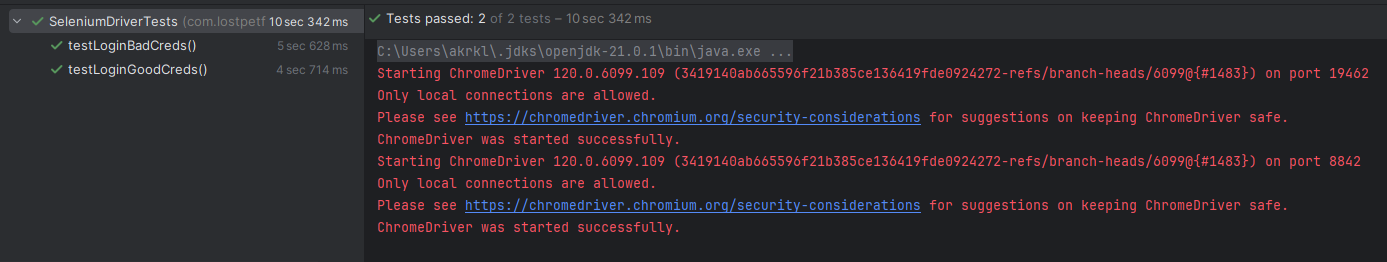
\includegraphics[width=\textwidth]{slike/test_passed.png}
	\caption{Testovi prolaze}
\end{figure}

\par\noindent\rule{\textwidth}{0.5pt}

\begin{figure}[!htb]
	\centering
	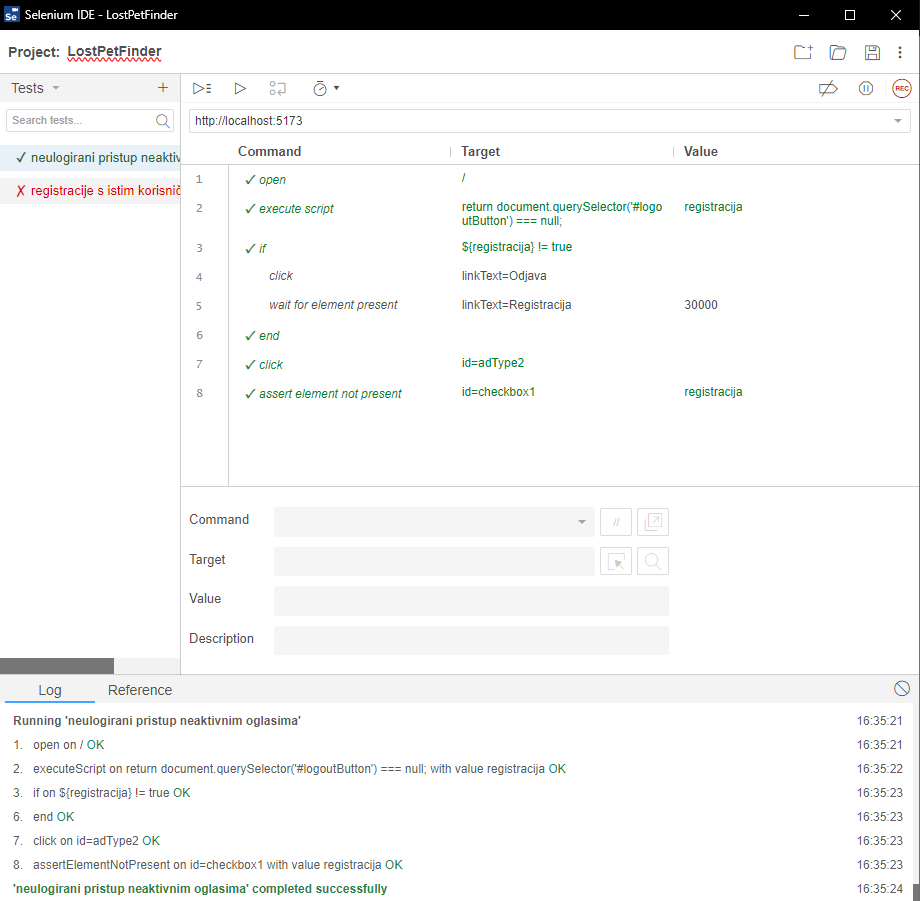
\includegraphics[width=\textwidth]{slike/selenium_test_1.png}
	\caption{Test: neulogirani korisnik pristupa neaktivnim oglasima}
\end{figure}

U ovom testu pomoću Selenium IDE-a provjerava se može li neulogirani korisnik pristupiti neaktivnim oglasima klikom na pripadajući radio button. Prvo se provjerava je li korisnik ulogiran, u tom slučaju se odjavljuje. Nakon toga se otvara stranica za prikaz oglasa, klikne se na radio button za prikaz neaktivnih oglasa i provjerava se je li se pojavio checkbox za filtriranje neaktivnih oglasa. Ako nije, test prolazi. Iz priloženog se vidi da aplikacija prolazi test.

\par\noindent\rule{\textwidth}{0.5pt}

\begin{figure}[!htb]
	\centering
	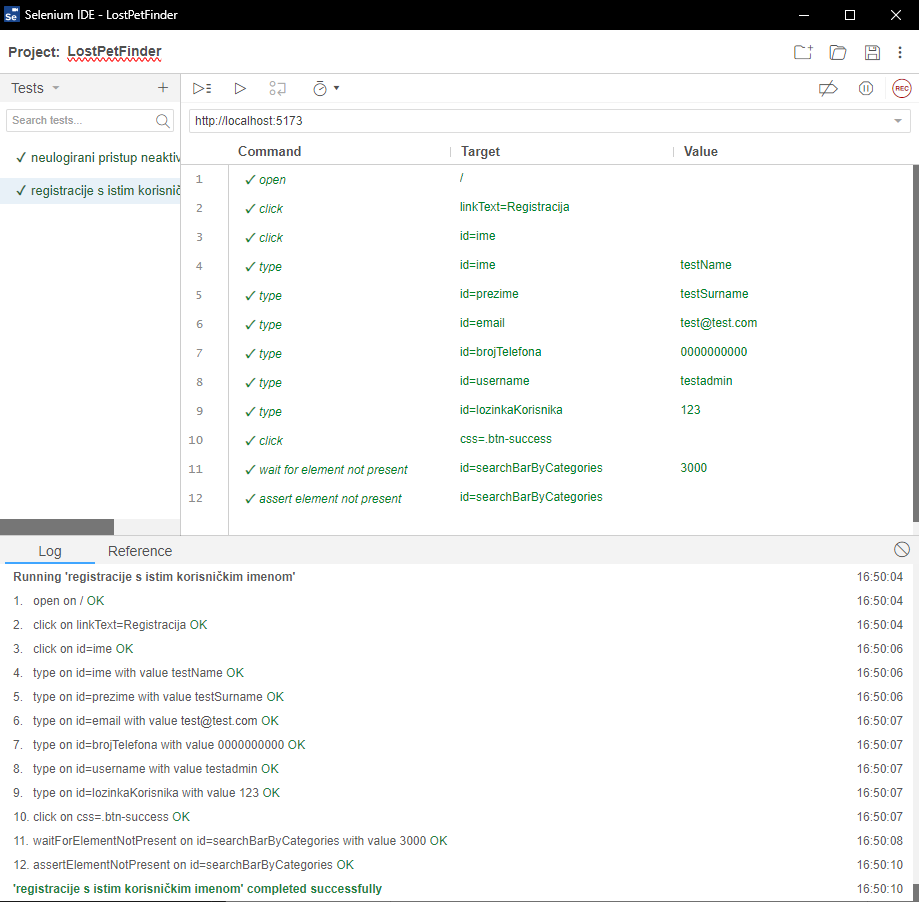
\includegraphics[width=\textwidth]{slike/selenium_test_2.png}
	\caption{Test: registracija s već postojećim podacima korisnika}
\end{figure}

U ovom testu pomoću Selenium IDE-a provjerava se kako aplikacija reagira na pokušaj registracije korisnika s podacima već postojećeg korisnika. Nakon unosa klikne se na gumb koji šalje formu i provjerava se je li se pojavio element za pretraživanje po kategorijama, odnosno je li se dogodio redirect na početnu stranicu. Ako nije, registracija nije uspjela i test prolazi. Iz priloženog se vidi da aplikacija prolazi test.

\eject


\section{Dijagram razmještaja}

\noindent Dijagrami razmještaja opisuju kako su komponente sustava raspoređene unutar njihovog radnog okruženja, uključujući sklopovlje i softversku podršku. Na poslužiteljskom računalu nalaze se web poslužitelj i poslužitelj baze podataka. Klijenti pristupaju web aplikaciji putem web preglednika. Arhitektura sustava temelji se na modelu "klijent-poslužitelj", gdje se komunikacija između računala korisnika (korisnik, registrirani korisnik, sklonište za životinje) i poslužitelja odvija preko HTTP veze.

\begin{figure}[!htb]
	\centering
	\includegraphics[width=\textwidth]{slike/Dijagram_razmještaja}
	\caption{Dijagram razmještaja}
\end{figure}

\eject

\section{Upute za puštanje u pogon}

\textbf{\textit{dio 2. revizije}}\\

\textit{Sljedeće upute prikazuju kako pustiti aplikaciju pogon pomoću servisa \underline{Render}\footnote{https://render.com/}.}

Izvorni kod aplikacije prvo treba pripremiti u svoj repozitorij na GitHubu (izradom forka repozitorija ove aplikacije) te bi trebalo izraditi korisnički račun na Renderu na koji treba povezati svoj GitHub račun. Nakon toga treba stvoriti novi poslužitelj na Renderu te u njega postaviti izvorni kod aplikacije. Za to je potrebno napraviti sljedeće korake:

\subsection{Izrada i postavljanje baze podataka aplikacije}

Proces izrade baze podataka je sljedeći:

\begin{enumerate}
	\item Na Render dashboardu odabrati \textit{New} -- \textit{PostgreSQL}.
	\item Popuniti polje \textit{Name} (proizvoljno).
	\item Odabrati \textit{PostgreSQL Version} -- 15.
	\item Odabrati tip stroja (za osnovnu funkcionalnost je dovoljan \textit{Free - 1 GB}).
	\item Odabrati \textit{Create Database}.
\end{enumerate}

Nakon što je baza podataka stvorena, potrebno je postaviti konfiguraciju backenda da se može povezati na nju. To se radi na sljedeći način:

\begin{enumerate}
	\item Na Render dashboardu odabrati bazu podataka nazvanu u prethodnom koraku.
	\item U kategoriji \textit{Info} pronaći skupinu \textit{Connections} u kojem se trebaju nalaziti sljedeća polja: \textit{Hostname}, \textit{Port}, \textit{Database}, \textit{Username}, \textit{Password} potrebna za idući korak.
	\item Na temelju tih podataka treba urediti/dodati segment u datoteci \textit{application.properties} koji se nalazi u direktoriju \textit{IzvorniKod/backend/src/main/resources} prema sljedećem obrascu:\\
	      \\
	      \verb+# Konfiguracija baze podataka+\\
	      \verb+spring.datasource.password=${DB_PASS:+\underline{\textlangle Password\textrangle}\verb+}+\\
	      \verb+spring.datasource.username=${DB_USERNAME:+\underline{\textlangle Username\textrangle}\verb+}+\\
	      \verb+spring.datasource.url=${DB_URL:jdbc:postgresql://+\underline{\textlangle Hostname\textrangle}\verb+:+\underline{\textlangle Port\textrangle}\verb+/+\underline{\textlangle Database\textrangle}\verb+}+
\end{enumerate}

\subsection{Puštanje u pogon backenda aplikacije}

Uz preduvjet da je baza podataka kreirana i konfigurirana ispravno, proces puštanja backenda u pogon je sljedeći:

\begin{enumerate}
	\item Na Render dashboardu odabrati \textit{New} -- \textit{Web Service}.
	\item Odabrati opciju \textit{Build and deploy from GitHub}.
	\item Odabrati repozitorij u kojem se nalazi izvorni kod aplikacije na povezanom GitHub računu pritiskom na tipku \textit{Connect} pokraj njega.
	\item Popuniti polje \textit{Name} s proizvoljnim imenom za backend.
	\item Odabrati odgovarajuću granu repozitorija u kojoj se nalazi izvorni kod aplikacije (obično je to \verb+main+).
	\item U polje \textit{Root Directory} upisati \verb+./IzvorniKod/backend+.
	\item Za \textit{Runtime} odabrati \textit{Docker}.
	\item Odabrati odgovarajući model računala u \textit{Instance Type}
	\item Na dnu stranice proširiti \textit{Advanced} opcije.
	\item U polje \textit{Dockerfile Path} upisati \verb+./Dockerfile+.
	\item Potvrditi izradu poslužitelja pritiskom na \textit{Create Web Service}.
	\item Nakon što se poslužitelj izradi, potrebno je kopirati adresu poslužitelja koja se nalazi ispod dodijeljenog imena poslužitelja nakon što se klikne na njega na Render dashboardu (adresa će biti potrebna pri konfiguraciji frontenda).
\end{enumerate}

\subsection{Puštanje u pogon frontenda aplikacije}

Nakon uspostavljanja backenda, sljedeći korak je puštanje u pogon frontenda. To se radi na sljedeći način:

\begin{enumerate}
	\item Na Render dashboardu odabrati \textit{New} -- \textit{Web Service}.
	\item Odabrati opciju \textit{Build and deploy from GitHub}.
	\item Odabrati repozitorij u kojem se nalazi izvorni kod aplikacije na povezanom GitHub računu pritiskom na tipku \textit{Connect} pokraj njega.
	\item Popuniti polje \textit{Name} s proizvoljnim imenom za frontend.
	\item Odabrati odgovarajuću granu repozitorija u kojoj se nalazi izvorni kod aplikacije (obično je to \verb+main+).
	\item U polje \textit{Root Directory} upisati \verb+./IzvorniKod/frontend+.
	\item Za \textit{Runtime} odabrati \textit{Node}.
	\item U polje \textit{Build Command} upisati \verb+yarn+.
	\item U polje \textit{Start Command} upisati \verb+yarn start-prod+.
	\item Odabrati odgovarajući model računala u \textit{Instance Type}.
	\item Potrebno je dodati dvije varijable okruženja u \textit{Environment Variables}:\\
	      \verb+API_BASE_URL+ s vrijednosti \verb+<Adresa poslužitelja backenda>+\\
	      \verb+PORT+ s vrijednosti \verb+5173+
\end{enumerate}

Nakon uspješnog postavljanja svih triju komponenti, aplikacija je spremna za korištenje te se može posjetiti na adresi koja je dodijeljena frontendu.


\eject